
Given, two circles with equations,
\begin{align}
S=\vec{x}^{T}\vec{x}-\myvec{4 & -5}\vec{x}-2=&0\label{rams/4/4/4/a/eq:1}\\
S'=\vec{x}^{T}\vec{x}-\myvec{5 & -6}\vec{x}=&0\label{rams/4/4/4/a/eq:2}
\end{align}
We know, the radical axis for the pair of circles, $S=0, S'=0$ is given by $L=S-S'=0$.\\
Using \eqref{rams/4/4/4/a/eq:1}, \eqref{rams/4/4/4/a/eq:2}, the required equation is
\begin{align}
\brak{\vec{x}^{T}\vec{x}-\myvec{4 & -5}\vec{x}-2}-\brak{\vec{x}^{T}\vec{x}-\myvec{5 & -6}\vec{x}=0}=&0\\
\myvec{1 & -1}\vec{x}-2=&0
\end{align}
$\therefore L=\myvec{1 & -1}\vec{x}-2=0$ is the equation of the required radical axis.  See Fig.  \ref{rams/4/4/4/a/plot}
\begin{figure}[!h]
 \centering
 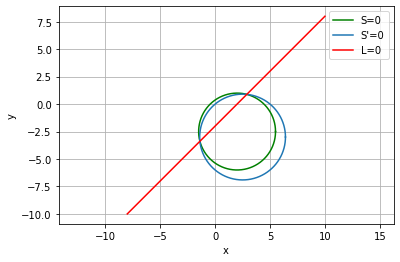
\includegraphics[width=\columnwidth]{solutions/4/4/4/a/figures/Assignment3.png}
 \caption{Pair of Circles and their radical axis}
 \label{rams/4/4/4/a/plot}
\end{figure}
